\section{Exploratory data analysis}

\subsection{Statistical analysis}
\begin{table}[h]
  \centering
  \begin{tabular}{|c|c|c|c|c|c|c|}
    \hline
      & n & mean & sd & median & trimmed & mad\\
    \hline
    CO(GT) & 191 & 2.748691 & 1.596801 & 2.50 & 2.560784 & 1.33434\\
    \hline
    PT08.S1(CO) & 200 & 1339.000000 & 255.446559 & 1332.50 & 1328.356250 & 233.50950\\
    \hline
    NMHC(GT) & 183 & 160.158470 & 139.745774 & 122.00 & 138.448980 & 118.60800\\
    \hline
    C6H6(GT) & 200 & 12.254000 & 8.274006 & 11.05 & 11.318750 & 7.33887\\
    \hline
    PT08.S2(NMHC) & 200 & 1016.950000 & 281.940276 & 1017.50 & 1005.556250 & 278.72880\\
    \hline
    NOx(GT) & 191 & 175.842932 & 94.999980 & 161.00 & 168.830065 & 85.99080\\
    \hline
    PT08.S3(NOx) & 200 & 1003.195000 & 278.431170 & 945.00 & 976.950000 & 234.99210\\
    \hline
    NO2(GT) & 191 & 115.612565 & 34.357971 & 119.00 & 116.549020 & 35.58240\\
    \hline
    PT08.S4(NO2)9 & 200 & 1671.040000 & 305.901187 & 1622.50 & 1641.750000 & 237.21600\\
    \hline
  \end{tabular}

  \begin{tabular}{|c|c|c|c|c|c|c|}
    \hline
      & min & max & range & skew & kurtosis & se\\
    \hline
    CO(GT) & 0.5 & 8.1 & 7.6 & 1.0755547 & 0.9704424 & 0.1155405\\
    \hline
    PT08.S1(CO) & 831.0 & 2040.0 & 1209.0 & 0.3506958 & -0.0955406 & 18.0627994\\
    \hline
    NMHC(GT) & 7.0 & 685.0 & 678.0 & 1.3200143 & 1.4422105 & 10.3303049\\
    \hline
    C6H6(GT) & 1.0 & 39.2 & 38.2 & 1.0086394 & 0.8567735 & 0.5850606\\
    \hline
    PT08.S2(NMHC) & 501.0 & 1754.0 & 1253.0 & 0.3211184 & -0.3339212 & 19.9361881\\
    \hline
    NOx(GT) & 16.0 & 478.0 & 462.0 & 0.6699740 & -0.0263597 & 6.8739573\\
    \hline
    PT08.S3(NOx) & 537.0 & 1918.0 & 1381.0 & 0.9745243 & 0.9172654 & 19.6880569\\
    \hline
    NO2(GT) & 28.0 & 194.0 & 166.0 & -0.2179968 & -0.4405303 & 2.4860555\\
    \hline
    PT08.S4(NO2) & 1134.0 & 2679.0 & 1545.0 & 0.9116828 & 0.7869557 & 21.6304804\\
    \hline
  \end{tabular}
\end{table}

\begin{table}[h]
  \centering
  \begin{tabular}{|c|c|c|c|c|c|c|}
    \hline
    & n & mean & sd & median & trimmed & mad\\
    \hline
    PT08.S5(O3) & 200 & 1233.2450000 & 389.2906253 & 1204.5000 & 1222.0375000 & 384.734700\\
    \hline
    T & 200 & 15.1965000 & 5.5702402 & 14.3000 & 14.8068750 & 5.189100\\
    \hline
    RH & 200 & 49.8030000 & 15.1352426 & 53.9000 & 50.6387500 & 15.270780\\
    \hline
    AH & 200 & 0.8085450 & 0.1059962 & 0.8125 & 0.8092338 & 0.104375\\
    \hline
    HIGH\_CO & 191 & 0.7225131 & 0.4489355 & 1.0000 & 0.7777778 & 0.000000\\
    \hline
    HIGH\_NMHC & 183 & 0.9945355 & 0.0739221 & 1.0000 & 1.0000000 & 0.000000\\
    \hline
    HIGH\_C6H6 & 200 & 0.6500000 & 0.4781665 & 1.0000 & 0.6875000 & 0.000000\\
    \hline
    HIGH\_NOx & 191 & 0.9947644 & 0.0723575 & 1.0000 & 1.0000000 & 0.000000\\
    \hline
    HIGH\_NO2 & 191 & 0.5968586 & 0.4918179 & 1.0000 & 0.6209150 & 0.000000\\
    \hline
  \end{tabular}
  
  \begin{tabular}{|c|c|c|c|c|c|c|}
    \hline
    & min & max & range & skew & kurtosis & se\\
    \hline
    PT08.S5(O3) & 384.0000 & 2359.0000 & 1975.0000 & 0.2942286 & -0.1157893 & 27.5270041\\
    \hline
    T & 6.1000 & 29.3000 & 23.2000 & 0.6005822 & -0.4670720 & 0.3938755\\
    \hline
    RH & 14.9000 & 81.1000 & 66.2000 & -0.4375140 & -0.8600569 & 1.0702233\\
    \hline
    AH & 0.5237 & 1.0945 & 0.5708 & 0.0279583 & -0.2727186 & 0.0074951\\
    \hline
    HIGH\_CO  & 0.0000 & 1.0000 & 1.0000 & -0.9861019 & -1.0329289 & 0.0324838\\
    \hline
    HIGH\_NMHC & 0.0000 & 1.0000 & 1.0000 & -13.3067908 & 176.0326973 & 0.0054645\\
    \hline
    HIGH\_C6H6 & 0.0000 & 1.0000 & 1.0000 & -0.6242595 & -1.6183168 & 0.0338115\\
    \hline
    HIGH\_NOx & 0.0000 & 1.0000 & 1.0000 & -13.6039602 & 184.0313314 & 0.0052356\\
    \hline
    HIGH\_NO2 & 0.0000 & 1.0000 & 1.0000 & -0.3918179 & -1.8561145 & 0.0355867\\
    \hline
  \end{tabular}  

  \caption{Summary statistics}
\end{table}


\begin{figure}[H]
  \centering
  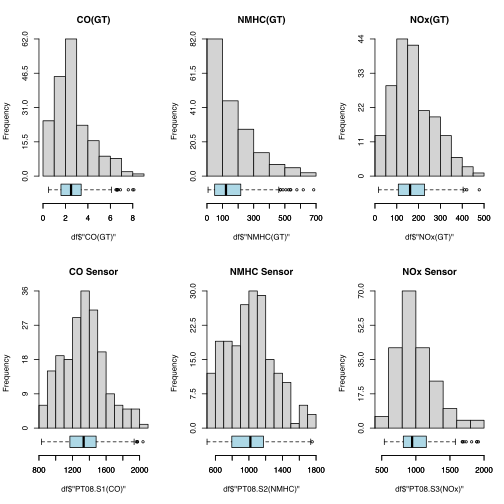
\includegraphics[width=0.7\textwidth]{figs/summary_1.png}
\end{figure}

\begin{figure}[H]
  \centering
  \includegraphics[width=0.7\textwidth]{figs/summary_2.png}
\end{figure}

\begin{figure}[H]
  \centering
  \includegraphics[width=0.5\textwidth]{figs/summary_3.png}
  \label{fig:summary}
  \caption{Summary of the data}
\end{figure}


\subsection{Correlation structure of the data}
\begin{figure}[H]
  \centering
  \includegraphics[width=0.5\textwidth]{figs/corr.png}
  \caption{Correlation matrix}
  \label{fig:corr}
\end{figure}

\begin{figure}[H]
  \centering
  \includegraphics[width=0.5\textwidth]{figs/scatter_matrix.png}
  \caption{Scatter matrix}
  \label{fig:scatter_matrix}
\end{figure}

%% analyze correlation
As can be seen in the two previous figures, the 10 first variables are correlated all together and the next 2 variables are also correlated together. The absloute humidity is isolated from the rest. This is a first clue that we can use to reduce the dimension of the data. We will use the PCA to reduce the dimension of the data.
The only variable collected by the sensors that is not correlated in the same with the others comes from the NOx sensor. Indeed, we can clearly dark red spot in the first figure and a linear relation in the other way on the second.

The variables relative to the humidity and temperature are much less correlated with the sensors varibles but much more within themselves. We can thus clearly see two groups of variables in the correlation matrix.

\subsection{Outlying observations using Mahalanobis distance}
\begin{figure}[H]
  \centering
  \includegraphics[width=0.5\textwidth]{figs/outliers.png}
  \caption{Mahalanobis distance outlier detection}
  \label{fig:mahalanobis}
\end{figure}

Using the \verb|outlier| function from \verb|pscyh| package, we can clearly distinguish the outliers from the dataset, which are the points that are not close to eachother.